\section{Models used for predicting outcomes of football matches}
\label{sec:background-models}

Already in 1982, \citeauthor{bib:maher-1982} presented a model for predicting the outcomes of football matches. Earlier studies in the field of football match result predictions used the negative binomial distribution to model the number of goals a given team will score during a given match. The earlier studies had rejected the Poisson model for predicting football results, stating that "chance does dominate the game" \citep{bib:maher-1982}. This assumption was shown wrong by \citet{bib:hill-1974}. Experts are able to accurately predict the final league standings before the league even start. According to \citet{bib:maher-1982}, this indicates that chance may play a considerable part in the results of a match, but differences in teams strengths and skills dominate in the long run.

A team's strength is usually divided into two separate strengths: attacking and defensive strengths. The attacking strength of a team represents the team's ability to score goals. The defensive strength of a team represents the team's ability to avoid conceding goals.

\subsection{The Poisson distribution}

\citet{bib:maher-1982} laid the foundation for several later prediction models when he presented his Poisson distribution model for predicting the number of goals scored by the the competing teams during a match. His model is based on the following assumption: each time a team has possession of the ball, there is an opportunity to attack, with the probability \textit{p} of scoring a goal. There are \textit{n} attacks during a match. If \textit{p} is constant, and the attacks are independent, the number of goals can be approximated using the Poisson distribution. \citet{bib:maher-1982} assumed that if team \textit{i} is playing at home against team \textit{j}, and the final scoreline is $(x_{ij}, y_{ij})$, then the final scoreline can be modelled using \cref{eq:maher-model}.
\begin{equation}
    \begin{aligned}
        X_{ij} \sim P(\alpha_{i}\beta_{j}) \\
        Y_{ij} \sim P(\gamma_{i}\delta_{j})
    \end{aligned}
    \label{eq:maher-model}
\end{equation}
\citet{bib:maher-1982} described that the variables represent different aspects of the match. A summary is given in \cref{tab:maher-model-description}.
\begin{table}
    \centering
    \noindent\begin{tabulary}{\textwidth}{C | L}
        \textbf{Variable}   & \textbf{What it represents} \\\hline
        $\alpha_{i}$        & The strength of team \textit{i}'s attack when playing at home \\
        $\beta_{j}$          & The weakness of team \textit{j}'s defence when playing away \\
        $\gamma_{i}$        & The weakness of team \textit{i}'s defence when playing at home \\
        $\delta_{j}$        & The strength of team \textit{j}'s attack when playing away \\
    \end{tabulary}
    \caption{The variables in the model of \citet{bib:maher-1982}.}
    \label{tab:maher-model-description}
\end{table}
The variables are based on the number of goals scored and conceded in the teams' earlier matches.

\subsubsection{Double Poisson distribution}

In the initial model of \citet{bib:maher-1982}, $X_{ij}$  and $Y_{ij}$ are assumed to be independent, "representing separate “games” at the two ends of the pitch". This is known as the double Poisson distribution.

Because of the independence, $\alpha$ and $\beta$ can be estimated for $x$ alone, whilst $\gamma$ and $\delta$ can be estimated from $y$ alone \citep{bib:maher-1982}. The log likelihood function for the home team's score can therefore be expressed as in \cref{eq:maher-log-likelihood}.
\begin{equation}
    log\ L(\alpha, \beta) = \sum_{i} \sum_{j \neq i} (-\alpha_{i} \beta_{j} + x_{ij}\ log(\alpha_{i}\beta_{j}) - log(x_{ij}!))
    \label{eq:maher-log-likelihood}
\end{equation}
Further, the maximum likelihood estimates, $\hat{\alpha}, \hat{\beta}$ can be shown to satisfy \cref{eq:maher-maximum-likelihood-estimates} \citep{bib:maher-1982}.
\begin{equation}
    \begin{aligned}
        \hat{\alpha_{i}} = \frac{\sum_{j \neq i} x_{ij}}{\sum_{j \neq i} \hat{\beta_{j}}} \\
        \hat{\beta_{j}} = \frac{\sum_{i \neq j} x_{ij}}{\sum_{i \neq j} \hat{\alpha_{i}}}
    \end{aligned}
    \label{eq:maher-maximum-likelihood-estimates}
\end{equation}
To determine the maximum likelihood estimates, \citet{bib:maher-1982} used the Newton-Raphson method. The similar was done for $\hat{\gamma}$ and $\hat{\delta}$. The determined estimates show the effects of the home ground advantage, as each team's attacking strength is significantly reduced when playing away \citep{bib:maher-1982}.

When evaluating his model, \citet{bib:maher-1982} used data from the four English Football League divisions for three consecutive years (1973-1975). \cref{fig:app-maher-strengths} shows the calculated team strengths for all teams in the English Division 1 1971-1972. \citet{bib:maher-1982} raised the question of whether using four different parameters for each team is really necessary. Using maximum likelihood estimates, \citet{bib:maher-1982} showed that the relative strengths of teams' attack and defense are the same whether playing at home or away, and that only $\alpha$ and $\beta$ are needed in order to make reasonable predictions. \citet{bib:maher-1982} then looked at the frequencies of goal scores scored in the English Division 1 over the three seasons. The results are shown in \cref{fig:app-maher-double-frequencies}. The model seems to underestimate the number of occasions where one and two goals are scored, while overestimating the number of times no goals or $\geq 4$ goals are scored \citep{bib:maher-1982}.

Even though the model has shown promising results, the assumptions behind it are not realistic \citep{bib:maher-1982}. \citet{bib:dixon-robinson-1998} showed how \textit{p} changes throughout the lifespan of a match. The scoring rate seems to increase throughout the game. \citet{bib:dixon-robinson-1998} pondered that the teams fatigue near the end of the match, making defensive mistakes, which in turn lead to goals. They also showed how the scoring rates are dependent on the current score. A lead to the home team tends to decrease their scoring rate, whilst increasing the scoring rate of the opposing team. A lead for the away team tends to increase the scoring rate of both teams.

\subsubsection{Bivariate Poisson distribution}

To accommodate the over-simplification of his model, \citet{bib:maher-1982} used the available data to create an improved, bivariate Poisson distribution model. In the new model, the marginal distributions are still Poisson with the same means as before, but a correlation factor, $\varrho$, is added between the scores. The new model can be thought of as considering the difference in the number of goals scored, $Z_{ij} = X_{ij} - Y_{ij}$, resulting in a model with two dependent parts \citep{bib:maher-1982}. One way to think of the bivariate Poisson distribution, according to \citet{bib:maher-1982}, is that
\begin{equation*}
    X_{ij} = U_{ij} + W_{ij} \quad \text{and} \quad Y_{ij} = V_{ij} + W_{ij},
\end{equation*}
where $U_{ij}$, $V_{ij}$ and $W_{ij}$ are independent Poisson with means $(\mu_{ij} - \eta_{ij})$, $(\lambda_{ij} - \eta_{ij})$ and $\eta_{ij}$, respectively. $\eta_{ij}$ being the co-variance between $X_{ij}$ and $Y_{ij}$. \citet{bib:maher-1982} experimented with different values for $\varrho$, and a value of $0.2$ yielded the best results. The bivariate version of his model improved the results considerably, compared to the initial model. \cref{fig:app-maher-bivariate-frequencies} shows the different frequencies for $Z_{ij}$ when applying the model to the English Division 1 1971-1972. One issue present in both the initial and improved models is the tendency to underestimate the number of drawn matches.

It is hard to say whether there is any correlation between the number of goals scored by each competing team. The question has been brought up in several studies. The assumption is, according to \citet{bib:maher-1982}, too simple to model reality. \citet{bib:karlis-ntzoufras-2003} argued that since two teams interact with each other during a match, the number of goals scored by each team are correlated. A change of style in play from one team will in turn change the probabilities of scoring a goal for both teams \citep{bib:karlis-ntzoufras-2003}. They supported their statements by analyzing data from the Champions League 2000-2001. \citet{bib:mchale-scarf-2007}, on the other hand, found little to no evidence of any correlation between the number of goals scored by the opposing teams. They used data from the English Premier League 2003-2006.

\citet{bib:karlis-ntzoufras-2003} built upon the model of \citet{bib:maher-1982}. They also used the bivariate Poisson distribution in their model. \citet{bib:karlis-ntzoufras-2003} modelled the number of goals scored in a match somewhat different from \citet{bib:maher-1982}. Instead of adding the correlation factor separately from the distribution, \citet{bib:karlis-ntzoufras-2003} added it to the distribution itself, resulting in a model of the form $(X_{ij}, Y_{ij}) \sim BP(\lambda_{i}, \lambda_{j}, \varrho)$, where
\begin{equation}
    \begin{aligned}
        log(\lambda_{i}) = \mu + H + \alpha_{i} + \beta_{j}
        \quad \text{and} \quad
        log(\lambda_{j}) = \mu + \alpha_{j} + \beta_{i}.
    \end{aligned}
    \label{eq:karlis-ntzoufras-model}
\end{equation}
$\lambda_{i}$ and $\lambda_{j}$ represent the expected number of goals scored for the home and away teams, respectively. $\varrho$ is the correlation factor, $\mu$ is a constant parameter, and $H$ is the home team effect parameter. $\alpha_{k}$ and $\beta_{i}$ represent the attacking and defensive abilities of team $k$, like in the model of \citet{bib:maher-1982}. $\mu$ represents the average number of goals scored per team when two teams of similar strengths play against each other.

Increasing the correlation between the number of goals scored improved the accuracy in prediction of draw games. \citet{bib:karlis-ntzoufras-2003} further improved their model by inflating the probability of drawn games. They stated that inflating the probability corrected a possible overdispersion of results. \cref{fig:app-karlis-ntzoufras-2003-results} shows the estimates for different versions of their model. Model 8, the diagonal inflated bivariate Poisson distributed model, shows the most promising results.

The model of \citet{bib:koopman-lit-2015} is also based on the bivariate Poisson distribution of \citet{bib:maher-1982}. Their model is similar to that of \citet{bib:karlis-ntzoufras-2003}:
\begin{equation*}
    (X_{ij}, Y_{ij}) \sim BP(\lambda_{i}, \lambda_{j}, \varrho),
\end{equation*}
where $\lambda_{i}$ and $\lambda_{j}$ are the intensity coefficients for $X$ and $Y$, and $\gamma$ is the coefficient that measures the dependence between $X_{ij}$ and $Y_{ij}$. $\lambda_{i}$ and $\lambda_{j}$ are allowed to vary over time. The intensities are then specified as
\begin{equation*}
    \begin{aligned}
        \lambda_{i, ijt} = exp(H + \alpha_{it} + \beta_{jt}) \\
        \lambda_{j, ijt} = exp(\alpha_{jt} + \beta_{it}),
    \end{aligned}
\end{equation*}
where $H$ is the home ground advantage coefficient and $\alpha_{kt}$ and $\beta_{kt}$ the attacking and defensive strengths of team $k$ in game week $t$. The attacking and defensive strengths are specified in \cref{eq:koopman-lit-team-strengths},
\begin{equation}
    \begin{aligned}
        \alpha_{it} = \mu_{\alpha, i}  + \phi_{\alpha, i}\ \alpha_{i, t-1} + \eta_{\alpha, it} \\
        \beta_{it} = \mu_{\beta, i}  + \phi_{\beta, i} \ \beta_{i, t-1} + \eta_{\beta, it}
    \end{aligned}
    \label{eq:koopman-lit-team-strengths}
\end{equation}
where $\mu_{\alpha, i}$ and $\mu_{\beta, i}$ are unknown constants, $\phi_{\alpha, i}$ and $\phi_{\beta, i}$ are auto-regressive coefficients, and $\eta_{\alpha, it}$ and $\eta_{\beta, it}$ are normally distributed independent error terms. $\alpha_{it}$ and $\beta_{it}$ are determined using the maximum likelihood estimator.

\citet{bib:koopman-lit-2015} applied their model in a betting setting. They used their predictions in combination with odds published at \citet{bib:football-data} for the English Premier League 2010-2012. During the evaluation, they used the Fixed bet strategy explained in \cref{sec:betting-strategies}, with a variable threshold $\tau$. \cref{fig:app-koopman-lit-threshold-levels} shows the effect $\tau$ has on the profitability of their system. With $\tau > 0.12$, the system is able to systematically gain a profit.


\subsubsection{Altered Poisson distribution models}

\citet{bib:dixon-coles-1997} used the initial model of \citet{bib:maher-1982} as basis for their model, with a small modification. The modified model included the home ground parameter, and can be seen in \cref{eq:dixon-coles-model}.
\begin{equation}
    \begin{aligned}
        X_{ij} \sim Poisson(\alpha_{i} \beta_{j} H) \\
        Y_{ij} \sim Poisson(\alpha_{j} \beta_{i}),
    \end{aligned}
    \label{eq:dixon-coles-model}
\end{equation}
where $\alpha_{k}$ and $\beta_{k}$ are the attacking and defensive strengths of team $k$, and $H$ the home ground advantage parameter. To improve the accuracy for low-scoring matches, \citet{bib:dixon-coles-1997} modified their model further, adding a dependence parameter. The new model can be seen in \cref{eq:dixon-coles-modified-model}.
\begin{equation}
    Pr(X_{ij} = x, Y_{ij} = y) = \tau_{\lambda, \mu}(x, y) \frac{\lambda^x exp(-\lambda)}{x!} \frac{\mu^y exp(-\mu)}{y!},
    \label{eq:dixon-coles-modified-model}
\end{equation}
where
\begin{equation}
    \begin{aligned}
        \lambda = \alpha_{i} \beta_{j} H \\
        \mu = \alpha_{j} \beta_{i}
    \end{aligned}
\end{equation}
and
\begin{equation}
    \tau_{\lambda, \mu}(x, y) =
    \begin{dcases}
        1 - \lambda \mu \varrho & \text{if } x = y = 0 \\
        1 + \lambda \varrho     & \text{if } x = 0, y = 1 \\
        1 + \mu \varrho         & \text{if } x = 1, y = 0 \\
        1 - \varrho             & \text{if } x = y = 1 \\
        1,                      & \text{otherwise}
    \end{dcases}.
\end{equation}
$\varrho$ is used as an dependence parameter. $\varrho = 0$ corresponds to independence. For $x \leq 1$ and $y \leq 1$, the independence distribution is altered.

Whilst the model of \citet{bib:maher-1982} incorporates static team strengths, \citet{bib:dixon-coles-1997} stated that recent results are more important than old ones to describe a team's current form. To incorporate this into their model, \citet{bib:dixon-coles-1997} scaled the contributions of older data, making recent data more significant. They also modified their model to enable inclusion of incomplete data sets and data from different leagues.

\citet{bib:rue-salvesen-2000} also used the initial model of \citeauthor{bib:maher-1982} as base for their work. They represent the attacking and defensive strengths of team $i$ as random variables $\alpha_{i}$ and $\beta_{i}$ respectively. Higher values imply greater strengths. They also represent $\mu_{\alpha, i}$ and $\sigma^2_{\alpha, i}$ as the prior mean and variance of $\alpha_{i}$, and similar for defence. $e_{i} = (\alpha, \beta)_{i}$ represents the properties of team $i$. \citet{bib:rue-salvesen-2000} also added a psychological effect, modelling the underestimation when a superior team meets a team that is of supposed inferior quality. The psychological effect is given as
\begin{equation*}
    \Delta_{ij} = (\alpha_{i} + \beta_{i} - \alpha_{j} - \beta_{j}) / 2,
\end{equation*}
and replaces the home ground advantage. However, \citet{bib:rue-salvesen-2000} propose the home ground advantage to be part of an extended version of their model. Another change from the model of \citet{bib:maher-1982} is the addition of a time factor, used to weigh the recent results above more distant results. In addition to the added variables, \citet{bib:rue-salvesen-2000} did some extra modifications to the model of \citet{bib:maher-1982}. They assumed that some of the information from the final scoreline comes from the league itself, and not the actual result. In a league where each team on average scores 1.23 goals per match, scoring 1 goal in a match is actually below the expected number of goals. To model this, \citet{bib:rue-salvesen-2000} used a variable, called $\epsilon$, which determines how much the league average should contribute to the predicted number of goals. This can be interpreted in the sense that only $(1 - \epsilon) * 100\%$ of the "information" in a match result is informative on $e_{i}$ and $e_{j}$ \citep{bib:rue-salvesen-2000}. Through experiments, they found that $\epsilon = 0.2$ yielded the best predictive results. They also observed that as one team scored a lot of goals, the probabilities diverted from the Poisson distribution. This was "solved" by clipping the number of goals scored at 5. Any number of goals scored above 5 did not count. That is, 8-2 is treated as 5-2, and 6-5 as 5-5. \citet{bib:rue-salvesen-2000} are not sure whether this is the best approach to solving the problem with diverting probabilities. Another mentioned solution is to reduce the scoreline until one get a more common one, i.e. from 7-4 to 5-2. By doing this, the information of the final result is kept, whilst removing the extra goals that do not provide important information \citep{bib:rue-salvesen-2000}. The system of \citet{bib:rue-salvesen-2000} is modelled as a Bayesian network. They added the use of Bayesian methods to update the estimates after each new match was played, and used Markov chain Monte Carlo techniques to draw inference from the network.

\citet{bib:rue-salvesen-2000} applied their model in a betting setting, using their strategy presented in \cref{sec:betting-strategies}. The cumulative profits for the English Premier League and Division 1 1997-1998 are shown in \cref{fig:app-rue-salvesen-profits}. As can be seen from the figure, the system was able to gain significant profits in both leagues, with a maximum profit of $250\%$ during the simulation. According to \citet{bib:rue-salvesen-2000}, the big spike in profits in the end of January was due to a single match, Manchester United versus Leicester City. The odds for an away-win was given at $13.8$, while the model predicted a probability of $0.184$ for the same outcome. The match ended $0-1$, resulting in a significant pay-off. In the end, the final profits were $39.6\%$ and $54.0\%$ respectively. Their system was able to win $42$ of the $112$ bets placed.

\subsubsection{Poisson difference distribution models}

In a later paper, \citet{bib:karlis-ntzoufras-2008} changed from using the bivariate Poisson distribution. They instead used the Poisson difference distribution. By doing this, they removed the effect of the correlation between the performance of the competing teams, and instead modelled the goal difference directly \citep{bib:karlis-ntzoufras-2008}. To model the goal difference, \citet{bib:karlis-ntzoufras-2008} calculated
\begin{equation*}
    Z_{ij} = X_{ij} - Y_{ij} \sim PD(\lambda_{i}, \lambda_{j}),
\end{equation*}
where $X_{ij}$ and $Y_{ij}$ are the Poisson distributions for the number of goals scored by the home team and away team, respectively. $Z_{ij}$ is then the distribution of the goal difference, and is called the Skellam's distribution (or Poisson difference distribution (PDD)) \citep{bib:karlis-ntzoufras-2008}. $\lambda_{i}$ and $\lambda_{j}$ are the model parameters, modelling the expected number of goals scored by each team, just like in \citet{bib:karlis-ntzoufras-2003}. The parameters are the same as defined in \cref{eq:karlis-ntzoufras-model}. \citet{bib:karlis-ntzoufras-2008} imposed two constraints on the attacking and defensive strengths of the teams, as given in \cref{eq:karlis-ntzoufras-constraints},
\begin{equation}
    \sum_{k=1}^{K} \alpha_{k} = 0 \quad \text{and} \quad \sum_{k=1}^{K} \beta_{k} = 0,
    \label{eq:karlis-ntzoufras-constraints}
\end{equation}
where $K$ is the number of competing teams. The attacking and defensive parameters can the be interpreted as the deviations from a team of moderate performance. Further, $H$ can then be interpreted as the expected goal difference in a match between two teams of the same attacking and defensive skills \citep{bib:karlis-ntzoufras-2008}. \citet{bib:karlis-ntzoufras-2008} authors show that the marginal distributions of $X$ and $Y$ are only Poisson distributed in special cases, and are in general defined as the convolution of a Poisson random variable with another discrete random variable, thus removing a large portion of the distributional assumptions concerning the number of goals scored by each team. This is one of the reasons they proposed the use of the Poisson difference distribution \citep{bib:karlis-ntzoufras-2008}. \citet{bib:karlis-ntzoufras-2008} then proceed to use Bayesian methods in order to incorporate any available information about each game via the prior distributions. Examples of mentioned relevant information are injuries, weather conditions and the fitness of the teams. Where no information is available, \citet{bib:karlis-ntzoufras-2008} proposed to use normal prior distributions for the parameters of the model, with mean equal to zero and a large variance (for example $10^4$). This is done to express prior ignorance \citep{bib:karlis-ntzoufras-2008}. The posterior predictive distributions are calculated using the Markov chain Monte Carlo algorithm.

According to \citet{bib:shahtahmassebi-moyeed-2016}, there are numerous limitations to the before-mentioned models utilizing the Poisson distribution. They cite \citet{bib:karlis-ntzoufras-2008}, supporting the use of goal difference instead of the number of goals scored. However, they address the drawback of overestimating the number of draws in the model of \citet{bib:karlis-ntzoufras-2008}. Another issue with the PDD is an issue with the double round-robin structure of most leagues. The home ground advantage results in distributions with one or both tails being too short or too long for the distribution \citep{bib:shahtahmassebi-moyeed-2016}. To overcome the limitations of the other Poisson-based models, \citet{bib:shahtahmassebi-moyeed-2016} used the generalized Poisson difference distribution (GPDD). The GPDD function is given in \cref{eq:gpdd-mass-function}.
\begin{equation}
    f_{GPDD}(Z = X - Y = z | \lambda_{1}, \lambda_{2}, \theta_{1}, \theta_{2}) = e^{-\lambda_{1} - \lambda_{2} - \theta_{1} z} \sum_{y=0}^{\infty} (\lambda_{1}, \theta_{1})_{z + y}\ (\lambda_{2}, \theta_{2})_{y}\ e^{-(\theta_{1} + \theta_{2})y}
    \label{eq:gpdd-mass-function}
\end{equation}
for any $z \in \mathbb{Z}$, where
\begin{equation*}
    (\lambda, \theta)_{x} = \frac{\lambda(\lambda + x \theta)^{x - 1}}{x!}.
\end{equation*}
$\lambda_{1}$ and $\theta_{1}$ refer to the positive half of the distribution, while $\lambda_{2}$ and $\theta_{2}$ refer to the negative half. The GPDD model can, just like the PDD model, be used for predicting the outcome of a match, but not the scoreline itself. The GPDD model, however, introduces more flexibility in its tails than the PDD model \citep{bib:shahtahmassebi-moyeed-2016}. To model the goal difference of a match, \citet{bib:shahtahmassebi-moyeed-2016} used the GPDD model as follows:
\begin{equation*}
    \begin{aligned}
        E(Z_{i}) = \mu_{i} = H + a_{h_{i}} - a_{v_{i}} \\
        Var(Z_{i}) = \sigma_{i}^{2} = \gamma_{1} + | a_{h_{i}} - a_{v_{i}} |,
    \end{aligned}
\end{equation*}
where $a_{h_{i}}$ and $a_{v_{i}}$ are the abilities of the home and visiting team in match $i$, $H$ is the home ground effect parameters (equal for all teams), and $\gamma_{1}$ is a positive constant for the variance. The variance is defined to increase with the difference in team abilities. \citet{bib:shahtahmassebi-moyeed-2016} imposed the constraint that all abilities sum to zero $(\sum_{k=1}^{K} a_{k} = 0)$. Furthermore, the values of $\theta_{1}$ and $\theta_{2}$ are assumed constant with respect to the team abilities. The values for $\lambda_{1}$ and $\lambda_{2}$ can be obtained using \cref{eq:shahtahmassebi-moyeed-lambda}.
\begin{equation}
    \begin{aligned}
        \lambda_{1, i} = \frac{[(1 - \theta_{2})^{2}\ \sigma_{i}^{2} + \mu_{i}] (1 - \theta_{1})^{3}}{(1 - \theta_{1})^{2} + (1 - \theta_{2})^{2}} \\
        \lambda_{2, i} = \frac{[(1 - \theta_{1})^{2}\ \sigma_{i}^{2} + \mu_{i}] (1 - \theta_{2})^{3}}{(1 - \theta_{1})^{2} + (1 - \theta_{2})^{2}}
    \end{aligned}    
    \label{eq:shahtahmassebi-moyeed-lambda}
\end{equation}
\citet{bib:shahtahmassebi-moyeed-2016} fitted the model in a Bayesian framework in order to incorporate any available information about each game via the prior distribution. The Bayesian approach allows for predicting match outcomes via the posterior predictive distribution, as well as for producing quantitative measures relating each team's performance. To generate samples for the posterior distribution, \citet{bib:shahtahmassebi-moyeed-2016} used the Markov chain Monte Carlo random walk Metropolis-Hastings algorithm. The model presented use the previous season as a baseline for the following season's results. \citet{bib:shahtahmassebi-moyeed-2016} state that teams generally at least intend to keep their position in the table from one season to the next. It is thus, according to the authors, realistic to use information from the previous season as prior information. For teams that are promoted and playing in the league for the first time, a non-informative normal prior distribution is assigned, like the one of \citet{bib:karlis-ntzoufras-2008}. The authors explain that this is done due to the nature of a football league: each team's abilities are measured relative to other teams in the same league. \citet{bib:shahtahmassebi-moyeed-2016} mention some issues with their final model. Firstly, using the previous season as baseline for the prior distributions may not be the optimal solution, as this does not allow for time-varying team abilities \citep{bib:shahtahmassebi-moyeed-2016}. They suggest an extension of the model would be to consider a dynamic model that supports varying team abilities, as well as a varying home ground advantage effect.

\subsection{Elo rating}

The ELO rating system is a rating system developed by for calculating the relative skills of players or teams in competitor-vs-competitor games, initially developed by Appard Elo. The system was initially developed for assessing the strengths of chess players, but have since been widely adopted for use in other sports \citep{bib:chessbase-2007}. The central assumption of the ELO rating system is that the performance of a competitor (either a person or a team) is a normally distributed random variable. Elo assumed the true skill level of a competitor to be the mean of this variable, and that the true skill level changes slowly over time. The skill level of a competitor serves as the basis for the competitor's ELO rating \citep{bib:chessbase-2007}.

\citet{bib:hvattum-arntzen-2010} used the ELO rating system in their model. Based on the results of previous matches, each team is assigned an ELO rating. This rating serves as a measure of the team's current strength. It should be noted that the computations of the ELO ratings need some initial ratings to be provided for each team, and that the ratings therefore can not be expected to be reliable before a sufficient number of matches have been taken into account \citep{bib:hvattum-arntzen-2010}.

Let $\ell_{i}^{H}$ and $\ell_{i}^{A}$ be the ratings of the home and away teams before a match at time $i$. A score system is defined, where points are rewarded to the teams after each match. The points awarded for a single match sum to 1. The expected score by the home and away teams are given by $\gamma^{H}$ and $\gamma^{A}$ respectively, where
\begin{equation*}
    \gamma^{H} = \frac{1}{1 + c^{(\ell_{i}^{A} - \ell_{i}^{H}) / d}} \quad \text{and} \quad
    \gamma^{A} = 1 - \gamma^{H} = \frac{1}{1 + c^{(\ell_{i}^{H} - \ell_{i}^{A}) / d}}.
\end{equation*}
$c$ and $d$ can be interpreted as setting the scaling of the rating \citep{bib:hvattum-arntzen-2010}. To calculate the ratings, the expected scores are compared to the observed scores, $\alpha^{H}$ and $\alpha^{A}$ respectively, given by
\begin{equation*}
    \alpha^{H} =
    \begin{dcases}
        1.0     & \text{if the home team wins} \\
        0.5     & \text{if the match is drawn} \\
        0,      & \text{otherwise}
    \end{dcases}
    \quad \text{and} \quad
    \alpha^{A} = 1 - \alpha^{H}.
\end{equation*}
The rating of the home team is updated after each match according to \cref{eq:hvattum-arntzen-rating-update}. The same is done for the away team rating.
\begin{equation}
    \ell_{i}^{H} = \ell_{i-1}^{H} + k (\alpha^{H} - \gamma^{H})
    \label{eq:hvattum-arntzen-rating-update}
\end{equation}

\citet{bib:hvattum-arntzen-2010} present two different versions of the ELO rating system. The first, referred to as the \textit{basic} ELO rating ($ELO_{b}$), set $k$ to be a constant parameter. The second, referred to as the $goal based$ ELO rating ($ELO_{g}$), replace $k$ with the expression $k = k_{0}(1 + \delta)^{\lambda}$, where $k_ {0}$ and $\lambda$ are constant parameters, and $\delta$ the absolute goal difference. The \textit{goal based} rating takes the goal difference in a match into account, rewarding a 3-0 win more strongly than a 2-1 win \citep{bib:hvattum-arntzen-2010}. According to \citet{bib:hvattum-arntzen-2010}, the values of $c$ and $d$ are not that important, as they only serve to set a scale of the ratings. Alternative values for $c$ and $d$ produce identical rating systems, but one have to set suitable values for $k$, $k_{0}$ and $\lambda$ \citep{bib:hvattum-arntzen-2010}. In their experiments, \citet{bib:hvattum-arntzen-2010} set $c=10$ and $d=400$, and calibrated the values of $k$, $k_{0}$ and $\lambda$ by minimizing the quadratic loss between the predicted values and the observed outcomes.

In order to use the ELO ratings for match prediction, \citet{bib:hvattum-arntzen-2010} make use of an ordered logit regression model \citep{bib:williams2006generalized}. An initial set of matches is used to compute initial ratings for all the teams in the league. A second set of matches is used to estimate the parameters of the model. The rating difference,
\begin{equation*}
    x = \ell_{i}^{H} - \ell_{i}^{A},
\end{equation*}
prior to the match serves as the covariate in the regression model. This system allows for updating both the ratings and the regression parameters, ensuring the most recent data is always utilized \citep{bib:hvattum-arntzen-2010}. 

The regression model serves as the basis for calculating the match predictions. The predictions are obtained by assigning the corresponding probability for each outcome of the match, resulting in a probability distribution for the three outcomes. \cref{fig:hvattum-arntzen-probabilities} shows the outcome probabilities as a function of the rating difference, given by the regression model at the end of the English Premier League 2006-2007. The home win and away win probabilities are equal when the rating difference is about -80. This shows how the model captures the home ground advantage \citep{bib:hvattum-arntzen-2010}.
\begin{figure}
    \centering
    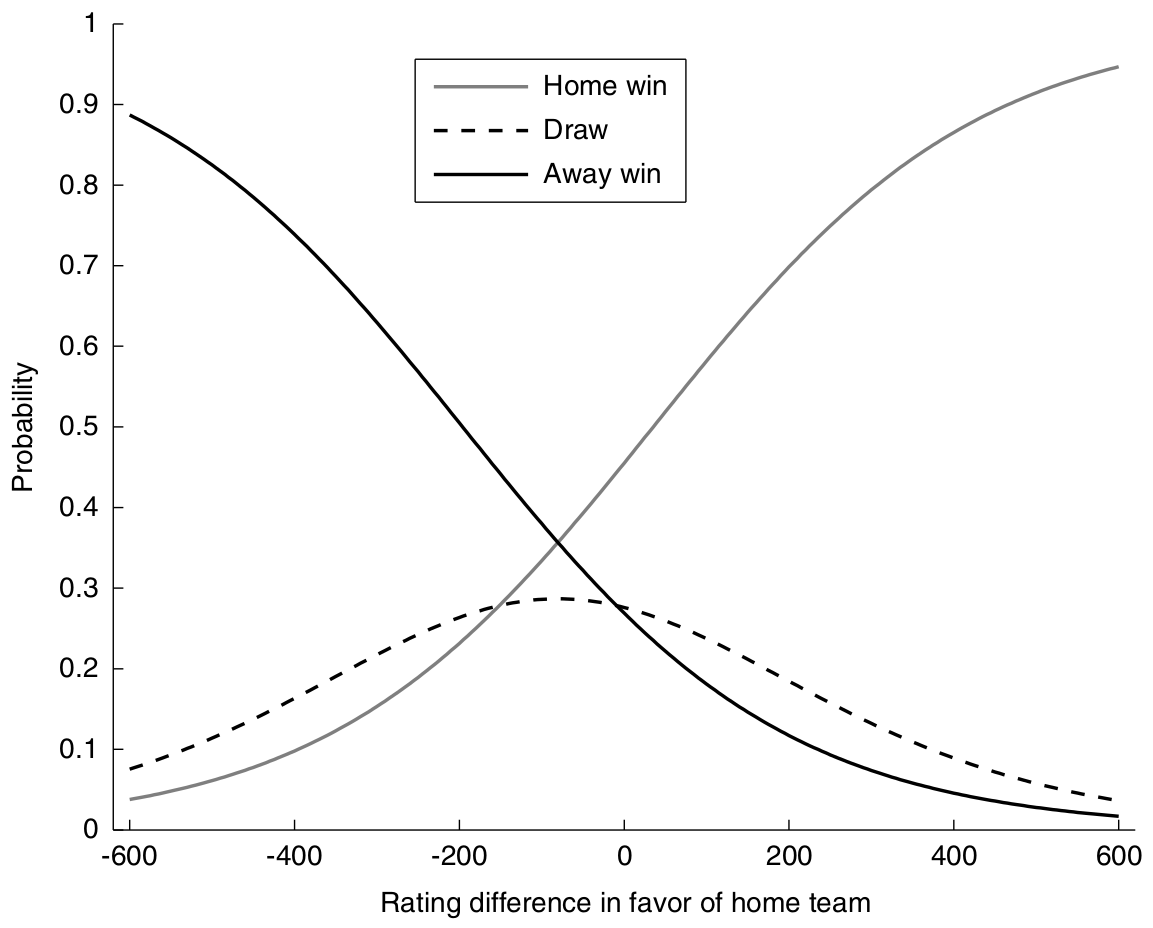
\includegraphics[width=0.8\textwidth]{state-of-the-art/hvattum-arntzen-probabilities.png}
    \caption{Outcome probabilities as a function of rating difference (in favor of home team), given by the regression model at the end of the English Premier League season 2006/2007. Taken from \citet{bib:hvattum-arntzen-2010}.}
    \label{fig:hvattum-arntzen-probabilities}
\end{figure}

\citet{bib:hvattum-arntzen-2010} evaluated their models in a betting setting. During the evaluation, they compared their models to other prediction models. The other prediction models include naive methods like assuming uniform probability of all outcomes (UNI), and basing the probabilities of observed past frequencies (FRQ). In addition, two versions of the model presented in \citet{bib:goddard-2005} were used (GOD\textsubscript{b}, GOD\textsubscript{g}). To compare the different models, \citet{bib:hvattum-arntzen-2010} used their predictions in combination with odds collected from various bookmakers. Match data from the English Premier League seasons 1993-2008 were used. The first two seasons were used for initial calculations of the ELO ratings. The five next seasons were used for estimating the parameters in the different prediction models. Finally, the eight remaining seasons were used for actual testing. \cref{fig:app-hvattum-arntzen-2010-profits} shows the total return for the different models. As can be seen, none of the presented models were able to gain a profit.

\subsection{Bradley–Terry modelling}

\citet{bib:cattelan-varin-firth-2013} built a prediction system using a dynamic Bradley-Terry model. The Bradley-Terry model is a probability model for predicting the outcome of a comparison. Given two individuals, $a$ and $b$, the model estimates the probability $P(a > b)$ using
\begin{equation}
    P(a > b) = \frac{p_{a}}{p_{a} + p_{b}},
    \label{eq:bradley-terry-model}
\end{equation}
where $p_{a}$ and $p_{b}$ are the scores assigned to $a$ and $b$ respectively. Here, $a > b$ can be read as "$a$ is preferred to $b$".

\citet{bib:cattelan-varin-firth-2013} use descriptors of the competing team's strengths as the basis for the scores. Two separate team strengths are calculated, one for matches played at home, one for matches played away. The strengths are calculated using earlier strengths and the number of points achieved in recent matches. In their model, \citet{bib:cattelan-varin-firth-2013} specify an evolution of a team's strengths depending only on past matches played of the same type. For home matches, the strength is estimated using \cref{eq:cattelan-varin-firth-home-strengths}.
\begin{equation}
    \alpha_{h_{i}}(t_{i}) = \lambda_{1} \mu_{h_{i}}(t_{i}) + (1 - \lambda_{1}) \alpha_{h_{i}}(t_{i-1}),
    \label{eq:cattelan-varin-firth-home-strengths}
\end{equation}
where $\alpha_{h_{i}}(t_{i})$ is the home strength of team $i$ at time $t_{i}$ and $t_{i-1}$ the time of the previous match played at home by team $h_{i}$. The term $\mu_{h_{i}}(t_{i})$ denotes the recent home strength of team $i$, based on the number of points earned in the last home match. $\mu_{h_{i}}(t_{i})$ is defined as
\begin{equation*}
    \mu_{h_{i}}(t_{i}) = \beta_{1} r_{h_{i}}(t_{i-1}),
\end{equation*}
where $\beta$ is a home-specific parameter, and $r_{h_{i}}(t_{i-1})$ the number of points earned in the last home match (3 for victory, 1 for draw, 0 for loss). $\lambda_{1} \in [0, 1]$ is used for determining how last result is weighted when estimating the team's home strength. The away strengths are estimated similarly, using away-specific parameters ($\lambda_{2}$ and $\beta_{2}$) instead of $\lambda_{1}$ and $\beta_{1}$.

To estimate the initial strengths, \citet{bib:cattelan-varin-firth-2013} assume that all teams start with equal home strength, $\beta_{1} \bar{r}_{h}$, where $\bar{r}_{h}$ is the average number of points gained at home in the previous season. $\alpha_{h_{i}}(t_{i})$ is then estimated using iterated back-substitution, thus incorporating the whole past of home matches \citep{bib:cattelan-varin-firth-2013}. The same goes for the away strength. The values of $\lambda_{1}$ and $\lambda_{2}$ are estimated using maximum profile likelihood estimation \citep{bib:cattelan-varin-firth-2013}.

To estimate the probabilities of each outcome, \citet{bib:cattelan-varin-firth-2013} use \cref{eq:cattelan-varin-firth-model}.
\begin{equation}
    P(Y_{i} \leq y_{i} | Y_{i-1} = y_{i-1}, ..., Y_{1} = y_{1}) = \frac{exp(\delta_{y_{i}} + \alpha_{h_{i}}(t_{i}) - \alpha_{v_{i}}(t_{i}))}{1 + exp(\delta_{y_{i}} + \alpha_{h_{i}}(t_{i}) - \alpha_{v_{i}}(t_{i}))},
    \label{eq:cattelan-varin-firth-model}
\end{equation}
where $y_{1} \in \{0, 1, 2\}$ denotes the outcome of the match ($2$ for home team victory, $1$ for draw and $0$ for away team victory). $\delta_{y_{i}}$ are cut-point parameters, where $\delta_{0} < \delta_{1} < \delta_{2}$. The cut-point parameters are needed for the Bradley-Terry model to support three outcomes. By setting $\delta_{0} = -\delta$ and $\delta_{1} = \delta$, with $\delta \geq 0$, one can ensure that two teams of the same strength playing at a neutral ground have the same probabilities of winning the match \citep{bib:cattelan-varin-firth-2013}.

When applying their model to the Italian Serie A 2008-2009, \citet{bib:cattelan-varin-firth-2013} concluded that their model seems to capture the relevant aspects of the evolution of team strengths. However, they find it reasonable to assume that using more information about the previous matches may result in improved predictions and more accurate forecasts.


\subsection{pi-football}
\label{subsec:pi-football}

The pi-football (probabilistic intelligence football) model \citep{bib:constantinou-fenton-neil-2012} is a Bayesian network model for predicting the outcomes of football matches, in the form of probabilities for each possible outcome (home win, draw, away win). The model is built up from mixing historical data with subjective expert knowledge. When building the model, the authors collected historical data from more than 6000 matches in the English Premier league from 1993 to 2010. The system was then used to predict the outcomes of all matches in the English Premier League 2010-2012, all of which are available online. The historical data is used to generate the model priors. A special feature of the pi-football model is the use of "anonymous" priors. That is, priors are predetermined by team-strength, not by distinct team names. Team strength is supplied as a ranked number representing the strength of a team for a particular season. The strength is based on a team's table position (using the number of accumulated points), separating the space of the league table into 14 levels. For example, the Manchester City match at home against Aston Villa the season of 2006-2007 is classified as a ranked 10 team at home against a ranked 8 team (with Manchester City totalling 42 points and Aston Villa totalling 50 points \citep{bib:constantinou-fenton-neil-2012}). The anonymous approach has several advantages \citep{bib:constantinou-fenton-neil-2012}:
\begin{itemize}
    \item It allows for making maximum use of limited data, as when predicting matches including newly-promoted teams.
    \item There is no need to ignore or weigh historical observations, as the system use the current strength of teams, and not their historical strengths.
    \item Historical observations do not need to be updated frequently, as there is a lot of historical data available.
    \item Data from one league can easily be adapted to work for another league, as the specific teams are not part of the model.
\end{itemize}

The model make use of four different factors to determine the abilities of a team:
\begin{enumerate}
    \item \textbf{Team strength}
    \item \textbf{Team form}
    \item \textbf{Team psychology}
    \item \textbf{Team fatigue}
\end{enumerate}
Factor 1 is the only objective factor in the model. It makes use of recent historical data to estimate of a team's current strength. The other three factors are used to revise the predictions made from factor 1. All factors are modelled as their own Bayesian network. The outcome of the three subjective factors are summarized in a single parameter, with a value from 0 to 1. A value of 0.5 signals no advantage to either team. A value of less than 0.5 signals an advantage to the home team. A value greater than 0.5 signals an advantage to the away team.

The network corresponding to factor 1 has three main components:
\begin{itemize}
    \item \textbf{Previous information:} Five parameters, each holding the number of pints accumulated the last five seasons. There is an increasing degree of uncertainty for the older seasons.
    \item \textbf{Current information:} A single parameter, holding a rough estimate of the team's current strength. Measured according to the number of points accumulated the current season and the expected number of points from the remaining matches. There is an increasing degree of uncertainty for the number of remaining matches.
    \item \textbf{Subjective information (optional):} Represented by a single parameter, holding an expert's subjective believed about the strength of a team. This is used to capture important events not captured by the historical data, such as the vast money usage by Manchester City the seasons from 2009 to 2012 (they spent £160m, £77m, £75m before the start of each seasons, respectively), improving their squad significantly.
\end{itemize}

The form of a team indicates a team's recent performance against its expectations. This is measured by comparing the team's expected performance against its observed performance during the five last game-weeks. The network of factor 2 determines whether one of the teams has better current form than the other, and has two main components:
\begin{itemize}
    \item \textbf{Current form:} Measured by a scale from 0 to 1. Scaled similarly to the subjective factors, indicating whether the team has over- or under performed according to its strength. Incorporates the home ground advantage; weights home form and general form ($\frac{2}{3}$ and $\frac{1}{3}$, respectively).
    \item \textbf{Availability of players resulted in current form:} The form is revised according to subjective factors including the availability of certain players, and the effect of returning first team players.
\end{itemize}

The network of factor 3 determines the difference in the psychological impact between the two teams, and has three main components:
\begin{itemize}
    \item \textbf{Head-to-head biases:} Models the psychological effect of head-to-head biases, such as local derbies.
    \item \textbf{Managerial impact:} Models any impact managerial issues might have on the team, such as recent change of manager.
    \item \textbf{Team spirit and motivation:} Models the current team spirit and motivation of the team.
\end{itemize}

Fatigue is determined by the toughness of the previous match, the number of days since that match, the number of first team players rested, and the participation of first team players in national team matches. The network of factor 4 has three main components:
\begin{itemize}
    \item \textbf{Restness:} The number of days since last match, along with information about resting first team players during that match. Gives an indication on how rested the team is.
    \item \textbf{Toughness of previous match:} The toughness of the previous match is also important in modelling a team's fatigue.
    \item \textbf{National team participation:} Can increase the fatigue by up to 50\%, depending on the level of participation of first team players in national team matches.
\end{itemize}

By combining the objective historical data with the subjective factors, the forecast prediction accuracy increased significantly, according to \citet{bib:constantinou-fenton-neil-2012}. They emphasise the importance of the quality of the expert's knowledge, claiming "...a perfect BN model would still fail to beat the bookmakers at their own game if the subjective expert inputs are inaccurate". With the weekly pressure to post their predictions online, the authors often had to get their subjective inputs from a team member, who "is certainly not an expert on the English premier League", resulting in inconsistent prediction accuracy \citep{bib:constantinou-fenton-neil-2012}. The authors also emphasise the importance of Bayesian networks, in which the subjective information easily can be represented and displayed.

\citet{bib:constantinou-fenton-neil-2012} applied their model in a betting setting. They used their predictions in combination with odds published at \citet{bib:football-data} for the English Premier League 2010-2011. In the evaluation, they used the Fixed bet strategy explained in \cref{sec:betting-strategies}, with a fixed threshold $\tau = 5\%$. 

The works of \citet{bib:constantinou-fenton-2013} show that the odds of a single bookmaker are not representative of the overall betting market. Therefore \citet{bib:constantinou-fenton-neil-2012} considered three different sets of odds when evaluating their system: the maximum odds available for each match outcome, the mean odds available for each outcome, and the odds specified by the most used bookmaker in the UK (representing $25\%$ of the total UK and Irish betting market \citep{bib:constantinou-fenton-neil-2012}), William Hill.

\cref{fig:app-constantinou-fenton-neil-2012-profits} shows the cumulative profits gained by the model using the different odds sets. As can be seen, the model was able to gain a profit for each of the different odds sets. Approximately $35\%$ of all placed bets were won. \cref{fig:app-constantinou-fenton-neil-2012-bets} show more detailed statistics for the three simulations. For $\tau = 5\%$, the model was able to generate a total profit of $14.19\%$ for the max odds set by the end of the season. By adjusting the value of $\tau$ to $11\%$, \citet{bib:constantinou-fenton-neil-2012} were able to increase the total profits to $35.63\%$.

\citet{bib:constantinou-fenton-neil-2012} suggest some extensions to the pi-football model. First, they mention a planned extension, exploring the effectiveness of the individual components used in their model. They hope this will help them understand how the specific components help in matching the bookmakers' odds. Another extension can explore whether revising the team strength itself (given subjective information), rather than the probability distribution, will improve the model's accuracy. Lastly, \citet{bib:constantinou-fenton-neil-2012} discuss exploring the impact of the time-dependent uncertainty when weighing the recent information. 